% pre1.tex
%
% Purpose:
%   Beamer report on the transmission-eigenvalue / Bloch-mode formulation
%   used in this repository for periodic waveguides and line-defect
%   scattering models.
%
% Main workflow:
%   The slides summarize the conceptual path from scalar Bloch theory, to
%   functional trace spaces, to Rayleigh wall coordinates, to one-cell Bloch
%   modes, to quasi-periodic Muller BIE scans and port trace matching.
%
% Based on:
%   notes/theory/bloch_ode.md, notes/theory/bloch_mode.md,
%   notes/theory/mode_selection.md, notes/theory/scat_formulation.md,
%   notes/theory/scat_formulation2.md, notes/theory/sol_representation.md,
%   notes/implementation/construct_A.md, and the top-level prototype scripts.
%
% Main differences:
%   This file is not a derivation note.  It is a concise presentation with
%   selected formulas and explicit placeholders for future numerical figures.
%
% Numerical goal:
%   Explain what has been assembled and what numerical results still need to
%   be inserted after MATLAB validation.

\documentclass[aspectratio=169]{beamer}

% Theme options:
% \usetheme{CambridgeUS}
% \usetheme{Madrid}
% \usetheme{Boadilla}
\usetheme{CambridgeUS}
\usecolortheme{dove}
\usefonttheme{professionalfonts}

\usepackage{amsmath}
\usepackage{amssymb}
\usepackage{bm}
\usepackage{graphicx}
\usepackage{tikz}
\usepackage{url}

\newcommand{\ii}{\mathrm{i}}
\newcommand{\Ccell}{\mathcal C}
\newcommand{\Aqp}{A_{\mathrm{QP}}}
\newcommand{\Atr}{\mathcal A}
\newcommand{\Dout}{D_{\mathrm{out}}}
\newcommand{\Nout}{N_{\mathrm{out}}}
\newcommand{\Din}{D_{\mathrm{in}}}
\newcommand{\Nin}{N_{\mathrm{in}}}
\newcommand{\sigmin}{\sigma_{\min}}
\newcommand{\FigurePlaceholder}[1]{%
  \begin{center}
    \setlength{\fboxsep}{1.2em}%
    \fbox{\parbox{0.75\textwidth}{\centering #1}}%
  \end{center}%
}
\newcommand{\SafeIncludeGraphics}[2][]{%
  \IfFileExists{#2}{%
    \includegraphics[#1]{#2}%
  }{%
    \FigurePlaceholder{Missing figure: \url{#2}}%
  }%
}

\title[TEP / Bloch Formulation]{Transmission Eigenvalue / Bloch-mode Formulation\\for Periodic Waveguides and Line Defects}
\author{}
\date{}

\AtBeginSection[]{
  \begin{frame}{Outline}
    \tableofcontents[currentsection]
  \end{frame}
}

\begin{document}

\begin{frame}
  \titlepage
\end{frame}

\begin{frame}{Outline}
  \tableofcontents
\end{frame}

\section{Motivation}

\begin{frame}{Motivation}
  \begin{itemize}
    \item The target PDEs are Helmholtz transmission problems in periodic waveguides and line-defect geometries.
    \item Two related workflows are studied: a TEP / eigenvalue formulation and a forced lead-scattering formulation.
    \item Dielectric inclusions impose transmission conditions; periodic half-leads impose exterior conditions.
    \item The exterior condition is a radiation/admissibility condition in the semi-infinite periodic leads. After eliminating the half-leads, this condition appears on the artificial ports as an outgoing trace condition.
  \end{itemize}
\end{frame}

\begin{frame}{Notation Schematic: One Row of Cells}
  \centering
  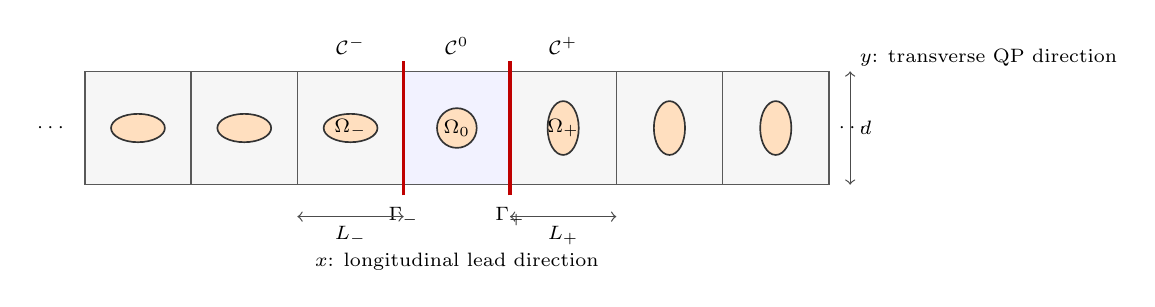
\begin{tikzpicture}[
    x=0.9cm,
    y=0.9cm,
    every node/.style={font=\scriptsize},
    cell/.style={draw=black!65, line width=0.5pt},
    leadcell/.style={fill=gray!7},
    centercell/.style={fill=blue!5},
    inclusion/.style={draw=black!80, fill=orange!25, line width=0.6pt},
    port/.style={draw=red!75!black, line width=1.1pt},
    dim/.style={<->, draw=black!70, line width=0.45pt}
  ]
    \foreach \x in {-5.25,-3.75,-2.25} {
      \draw[cell, leadcell] (\x,-0.8) rectangle ++(1.5,1.6);
      \draw[inclusion] (\x+0.75,0) ellipse [x radius=0.38, y radius=0.20];
    }

    \draw[cell, centercell] (-0.75,-0.8) rectangle (0.75,0.8);
    \draw[inclusion] (0,0) circle [radius=0.28];

    \foreach \x in {0.75,2.25,3.75} {
      \draw[cell, leadcell] (\x,-0.8) rectangle ++(1.5,1.6);
      \draw[inclusion] (\x+0.75,0) ellipse [x radius=0.22, y radius=0.38];
    }

    \draw[port] (-0.75,-0.95) -- (-0.75,0.95);
    \draw[port] (0.75,-0.95) -- (0.75,0.95);

    \node[above] at (-1.5,0.9) {$\mathcal C^-$};
    \node[above] at (0,0.9) {$\mathcal C^0$};
    \node[above] at (1.5,0.9) {$\mathcal C^+$};

    \node[below] at (-0.75,-0.98) {$\Gamma_-$};
    \node[below] at (0.75,-0.98) {$\Gamma_+$};

    \node at (-1.5,0) {$\Omega_-$};
    \node at (0,0) {$\Omega_0$};
    \node at (1.5,0) {$\Omega_+$};

    \draw[dim] (-2.25,-1.25) -- (-0.75,-1.25);
    \node[below] at (-1.5,-1.25) {$L_-$};
    \draw[dim] (0.75,-1.25) -- (2.25,-1.25);
    \node[below] at (1.5,-1.25) {$L_+$};

    \draw[dim] (5.55,-0.8) -- (5.55,0.8);
    \node[right] at (5.55,0) {$d$};
    \node[below] at (0,-1.62) {$x$: longitudinal lead direction};
    \node[right] at (5.55,1.0) {$y$: transverse QP direction};

    \node[left] at (-5.35,0) {$\cdots$};
    \node[right] at (5.25,0) {$\cdots$};
  \end{tikzpicture}

  \vspace{0.7em}
  \small
  Only the longitudinal cell chain is drawn. The longitudinal lead periods
  are \(L_-\) and \(L_+\). The transverse quasiperiodic period is \(d\).
\end{frame}

\begin{frame}{Reference Cells and Ports}
  \begin{itemize}
    \item The three central reference cells are
    \[
      \Ccell^-, \qquad \Ccell^0, \qquad \Ccell^+ .
    \]
    \item The center cell contains the dielectric inclusion
    \[
      \Omega_0, \qquad \Sigma=\partial\Omega_0 .
    \]
    \item The artificial center-cell boundaries are
    \[
      \Gamma_-=\{x=X_-\}, \qquad
      \Gamma_+=\{x=X_+\}.
    \]
    \item Port outward normals are
    \[
      \nu_{\Gamma_-}=-e_x, \qquad \nu_{\Gamma_+}=+e_x .
    \]
  \end{itemize}
\end{frame}

\section{Problem Formulation}

\begin{frame}{Helmholtz Transmission Model}
  The scalar model is a Helmholtz transmission problem:
  \[
    (\Delta+k^2n^2(x))u=0.
  \]
  Equivalently, in a background region and inside a dielectric inclusion,
  \[
    (\Delta+k_e^2)u_e=0,
    \qquad
    (\Delta+k_i^2)u_i=0.
  \]
  When
  \[
    k_i=n k_e,
  \]
  the parameter \(n\) is the refractive index of the dielectric inclusion relative to the background.
\end{frame}

\begin{frame}{Transmission Conditions on Inclusions}
  For every dielectric inclusion boundary
  \[
    \Sigma_j=\partial\Omega_j,
  \]
  impose
  \[
    u_e=u_i,
    \qquad
    \partial_\nu u_e=\partial_\nu u_i
    \quad \text{on } \Sigma_j.
  \]
  \begin{block}{Where this applies}
    Transmission conditions apply on all dielectric cylinders or inclusions, not only on the center obstacle.
  \end{block}
\end{frame}

\begin{frame}{Where the Transmission Conditions Appear}
  If the finite center region contains several dielectric inclusions, all of their boundaries carry the same transmission conditions.
  In the periodic leads, those conditions are already encoded in the lead-cell scattering and trace-propagation computation.
  In the current center-obstacle formulation,
  \[
    \Sigma=\partial\Omega_0
  \]
  is the explicit center inclusion boundary used in the M\"uller BIE row.
\end{frame}

\begin{frame}{TEP / Eigenvalue-type Problem}
  For fixed quasiperiodicity \(\beta\), seek a nonzero field and spectral parameter \(k\) such that:
  \begin{itemize}
    \item Helmholtz equations hold in the background and in all inclusions.
    \item Transmission conditions hold on all inclusion boundaries.
    \item The field is \(y\)-quasiperiodic:
    \[
      u(x,y+d)=e^{\ii\beta d}u(x,y).
    \]
    \item The left and right semi-infinite periodic leads satisfy radiation/admissibility conditions at infinity.
  \end{itemize}
\end{frame}

\begin{frame}{Homogeneous Matrix Form}
  After eliminating the half-leads, the radiation/admissibility condition becomes outgoing trace conditions on the artificial ports.
  The eigenvalue-type system is homogeneous:
  \[
    \mathcal A(k,\beta)x=0.
  \]
  In the simpler 1D periodic prototype, this reduces to the boundary equation
  \[
    A_{\mathrm{QP}}(k,\beta)\eta=0.
  \]
  Candidate eigenvalues are detected by
  \[
    \sigma_{\min}(A_{\mathrm{QP}}(k,\beta))\approx 0,
    \qquad
    \sigma_{\min}(\mathcal A(k,\beta))\approx 0.
  \]
\end{frame}

\begin{frame}{Forced Lead-scattering Problem}
  For fixed \(k\) and \(\beta\), prescribe legal incoming port coefficients
  \[
    p_{\mathrm{in}}^-,
    \qquad
    p_{\mathrm{in}}^+.
  \]
  Solve for:
  \begin{itemize}
    \item the field in the finite defect or center region;
    \item internal fields in dielectric inclusions;
    \item outgoing scattered trace coefficients \(r^-\) and \(r^+\).
  \end{itemize}
  This is a forced problem, not an eigenvalue search.
\end{frame}

\begin{frame}{Forced Matrix Form}
  The scattering system is
  \[
    \mathcal A(k,\beta)x=b_{\mathrm{in}}.
  \]
  The right-hand side is built from legal incoming traces:
  \[
    b_{\mathrm{in}}
    =
    \begin{bmatrix}
      0\\
      D_{\mathrm{in}}^-p_{\mathrm{in}}^-\\
      N_{\mathrm{in}}^-p_{\mathrm{in}}^-\\
      D_{\mathrm{in}}^+p_{\mathrm{in}}^+\\
      N_{\mathrm{in}}^+p_{\mathrm{in}}^+
    \end{bmatrix}.
  \]
\end{frame}

\begin{frame}{TEP Versus Scattering}
  \begin{block}{TEP / eigenvalue-type problem}
    Homogeneous system. The goal is to find \(k\) where a nontrivial admissible field exists.
  \end{block}
  \begin{block}{Lead-scattering problem}
    Forced system at fixed \(k,\beta\). The goal is to solve the response to legal incoming port data.
  \end{block}
  Both workflows use the same trace machinery, but the right-hand side and numerical target are different.
\end{frame}

\section{Bloch Theory}

\begin{frame}{ODE Transfer Matrix Warm-up}
  For a periodic scalar ODE,
  \[
    -u''(x)+q(x)u(x)=k^2u(x),
    \qquad q(x+d)=q(x),
  \]
  set
  \[
    U(x)=\begin{bmatrix}u(x)\\ u'(x)\end{bmatrix}.
  \]
  One-period propagation is
  \[
    U(d)=M(k)U(0).
  \]
\end{frame}

\begin{frame}{ODE Floquet Multiplier}
  Let \(\Phi(x;k)\) be the fundamental matrix:
  \[
    U(x)=\Phi(x;k)U(0),
    \qquad
    \Phi(0;k)=I.
  \]
  The one-period monodromy matrix is
  \[
    M(k)=\Phi(d;k).
  \]
  A Bloch solution satisfies
  \[
    U(d)=\lambda U(0).
  \]
  Hence the initial Cauchy data
  \[
    v=U(0)
  \]
  must solve
  \[
    M(k)v=\lambda v,
    \qquad
    v=U(0).
  \]
\end{frame}

\begin{frame}{Waveguide Trace Space Before Coordinates}
  In a waveguide, the wall data are not initially finite vectors.
  For a vertical section \(\Gamma_\star\), the natural Cauchy trace has the form
  \[
    \operatorname{Tr}_{\Gamma_\star}u
    =
    \begin{bmatrix}
      u|_{\Gamma_\star}\\
      \partial_{\nu_{\Gamma_\star}}u|_{\Gamma_\star}
    \end{bmatrix}
    \in
    H^{1/2}(\Gamma_\star)\times H^{-1/2}(\Gamma_\star).
  \]
  Bloch-mode matching starts from this infinite-dimensional trace space.
\end{frame}

\begin{frame}{Rayleigh Wall Basis from Quasiperiodicity}
  Write the quasiperiodic field as
  \[
    u(x,y)=e^{\ii\beta y}v(x,y),
    \qquad
    v(x,y+d)=v(x,y).
  \]
  For a fixed wall \(x=X\), \(v(X,y)\) is periodic, so it has a Fourier expansion.
  This gives
  \[
    \beta_m=\beta+\frac{2\pi m}{d},
    \qquad
    \psi_m(y)=\frac{1}{\sqrt d}e^{\ii\beta_m y}.
  \]
  This page is only about Fourier coordinate representation of quasiperiodic wall traces.
  It is not yet Bloch theory.
\end{frame}

\begin{frame}{Truncated Trace Coordinates}
  After truncation to \(|m|\le M\), set
  \[
    K=2M+1.
  \]
  A port trace is represented by coefficient vectors
  \[
    D^\pm\in\mathbb C^K,
    \qquad
    N^\pm\in\mathbb C^K.
  \]
  Thus the truncated Cauchy trace lives in
  \[
    \mathbb C^K\times\mathbb C^K.
  \]
  On \(\Gamma_-\), \(N^-\) means \(-\partial_x u\); on \(\Gamma_+\), \(N^+\) means \(+\partial_x u\).
\end{frame}

\begin{frame}{Rayleigh Coordinates Are Not Bloch Modes}
  \begin{itemize}
    \item \(\psi_m\) are wall coordinate functions.
    \item A Bloch mode is a one-cell propagation or scattering eigenmode.
    \item A Bloch mode can be spatially complicated inside a lead cell.
    \item Its wall trace can still be written in Rayleigh coordinates.
  \end{itemize}
  The useful separation is
  \[
    \text{Rayleigh basis}=\text{trace coordinates},
    \qquad
    \text{Bloch mode}=\text{cell eigenmode}.
  \]
\end{frame}

\begin{frame}{Why Compute Bloch Modes?}
  \begin{itemize}
    \item The Rayleigh basis only gives coordinates in
    \(\mathbb C^K\times\mathbb C^K\).
    \item Algebraically, many chosen Cauchy trace subspaces could close the
    finite port-matching system.
    \item The Bloch computation selects the physically admissible subspaces
    \(E_{\mathrm{in}}^\pm\) and \(E_{\mathrm{out}}^\pm\) coming from the
    semi-infinite periodic leads.
    \item An arbitrary trace subspace would impose an artificial port
    condition and generally solve a different problem.
  \end{itemize}
  \[
    \boxed{\text{Bloch modes identify the physical admissible trace subspaces.}}
  \]
  Once \(E_{\mathrm{out}}^\pm\) is selected, its Bloch eigenvectors may be
  replaced by any well-conditioned basis of the same subspace.
\end{frame}

\begin{frame}{One Lead Cell: Wall Amplitudes}
  Near the left wall of a lead cell,
  \[
    u(x,y)
    =
    \sum_m a_m^L e^{\ii\gamma_m(x-X_L)}\psi_m(y)
    +
    \sum_m b_m^L e^{-\ii\gamma_m(x-X_L)}\psi_m(y).
  \]
  Near the right wall, use amplitudes \(a^R\) and \(b^R\).
  The four vectors mean:
  \[
    a^L:\text{ right-going at left wall},\quad
    b^L:\text{ left-going at left wall},
  \]
  \[
    a^R:\text{ right-going at right wall},\quad
    b^R:\text{ left-going at right wall}.
  \]
\end{frame}

\begin{frame}{Cell Scattering Matrix}
  The one-cell scattering matrix maps incoming wall amplitudes to outgoing wall amplitudes:
  \[
    \begin{bmatrix} b^L\\ a^R \end{bmatrix}
    =
    S_{\mathrm{cell}}
    \begin{bmatrix} a^L\\ b^R \end{bmatrix}
    =
    \begin{bmatrix}
      R_L & T_{R\to L}\\
      T_{L\to R} & R_R
    \end{bmatrix}
    \begin{bmatrix} a^L\\ b^R \end{bmatrix}.
  \]
  This replaces the scalar ODE transfer matrix in a waveguide cell.
\end{frame}

\begin{frame}{Bloch Condition in the Cell}
  As in the ODE case, a Bloch mode is found by requiring the two wall traces of one cell to satisfy a Floquet relation.
  This is the wall-trace version of
  \[
    U(d)=\lambda U(0).
  \]
  For a multiplier \(\lambda\) from left to right, impose
  \[
    a^R=\lambda a^L,
    \qquad
    b^R=\lambda b^L.
  \]
  With \(a=a^L\) and \(b=b^L\), substitution into the scattering relation gives
  \[
    A_{\mathrm{sc}}
    \begin{bmatrix}a\\b\end{bmatrix}
    =
    \lambda B_{\mathrm{sc}}
    \begin{bmatrix}a\\b\end{bmatrix}.
  \]
  This is the one-cell Bloch generalized eigenproblem.
\end{frame}

\begin{frame}{Generalized Eigenproblem Blocks}
  One convenient block form is
  \[
    A_{\mathrm{sc}}
    =
    \begin{bmatrix}
      -R_L & I\\
      T_{L\to R} & 0
    \end{bmatrix},
    \qquad
    B_{\mathrm{sc}}
    =
    \begin{bmatrix}
      0 & T_{R\to L}\\
      I & -R_R
    \end{bmatrix}.
  \]
  The eigenvector is
  \[
    z=
    \begin{bmatrix}a\\b\end{bmatrix},
    \qquad
    A_{\mathrm{sc}}z=\lambda B_{\mathrm{sc}}z.
  \]
\end{frame}

\begin{frame}{Dispersion in a Homogeneous Rayleigh Exterior}
  For a homogeneous exterior with \(y\)-quasiperiodic period \(d\),
  \[
    \beta_m=\beta+\frac{2\pi m}{d},
    \qquad
    \gamma_m^2=k^2-\beta_m^2.
  \]
  The open \(x\)-direction factor is controlled explicitly by \(\gamma_m\).
  \begin{block}{Rayleigh light-line criterion}
    \[
      \boxed{
      \text{Rayleigh order }m\text{ decays in the open }x\text{-direction}
      \iff
      k<|\beta_m|
      }
    \]
  \end{block}
  If \(k>|\beta_m|\), that order is propagating/radiating. The cutoff
  \(k=|\beta_m|\) is a grazing light-line case and is numerically delicate.
\end{frame}

\begin{frame}{Periodic Leads: Dispersion Is Implicit}
  In a periodic half-lead, Rayleigh functions are still useful wall trace
  coordinates, but a physical Bloch mode is not a single Rayleigh order.
  It is obtained from the lead-cell eigenproblem:
  \[
    A_{\mathrm{sc}}(k,\beta)z
    =
    \lambda B_{\mathrm{sc}}(k,\beta)z.
  \]
  The multiplier \(\lambda_j(k,\beta)\) is the one-cell propagation factor.
  \begin{block}{Periodic-lead dispersion}
    The admissible decaying/outgoing components are selected only after
    fixing \((k,\beta)\) and solving the cell eigenproblem.
  \end{block}
\end{frame}

\begin{frame}{Intuition for Choosing the Rayleigh Truncation \(M\)}
  \footnotesize
  \begin{block}{Artificial-wall trace vs. physical coupling}
    The wall \(\Gamma_\pm\) is a coordinate section, not a material interface.
    Strict wall-trace accuracy is stronger than resolving the coupling that
    survives from one inclusion to the next.
  \end{block}
  Suppose an inclusion boundary is at least a distance \(\delta\) from each
  vertical cell wall. Adjacent inclusions are then separated by roughly
  \(2\delta\) through homogeneous background.
  For high-order evanescent Rayleigh components,
  \[
    \gamma_m\approx \ii|\beta_m|,
    \qquad
    \text{propagation over }\ell:\ e^{-\operatorname{Im}\gamma_m\ell}.
  \]
  \[
    \text{wall-trace tail: } e^{-\operatorname{Im}\gamma_m\delta},
    \qquad
    \text{inter-inclusion coupling tail: } e^{-2\operatorname{Im}\gamma_m\delta}.
  \]
  The same intuition applies to eigenvalue formulations: a nontrivial density
  on \(\Omega_0\) still couples through the same Rayleigh/Floquet trace
  machinery.
  \begin{alertblock}{Practical guideline, not a theorem}
    Use \(M\) to resolve effective inter-inclusion near-field coupling.
    Near resonances, band edges, grazing modes, or ill-conditioned systems,
    verify the choice by \(M\)-convergence tests.
  \end{alertblock}
\end{frame}

\section{Radiation Condition and Trace Spaces}

\begin{frame}{What Counts as a Bloch Mode}
  A Bloch mode is one selected eigenmode of the one-cell problem:
  \[
    A_{\mathrm{sc}}z_j=\lambda_j B_{\mathrm{sc}}z_j.
  \]
  Its multiplier \(\lambda_j\) describes propagation across one lead period.
  In the simple propagating notation,
  \[
    \lambda_j=e^{\ii\alpha_j L_\pm}.
  \]
  This term should be reserved for these Floquet multiplier eigenmodes.
\end{frame}

\begin{frame}{Incoming Wave Versus One Mode}
  A general incoming wave is usually a linear combination in an incoming trace subspace:
  \[
    \begin{bmatrix}
      D_{\mathrm{in}}^\pm p_{\mathrm{in}}^\pm\\
      N_{\mathrm{in}}^\pm p_{\mathrm{in}}^\pm
    \end{bmatrix}.
  \]
  It is a single Bloch mode only if \(p_{\mathrm{in}}^\pm\) selects exactly one eigenmode basis vector.
  Otherwise it is a legal incoming trace, not one mode.
\end{frame}

\begin{frame}{Port Trace Bases on \(\Gamma_\pm\)}
  The matrices
  \[
    D_{\mathrm{in}}^\pm,\quad
    N_{\mathrm{in}}^\pm,\quad
    D_{\mathrm{out}}^\pm,\quad
    N_{\mathrm{out}}^\pm
  \]
  are defined on the center-cell artificial boundaries
  \[
    \Gamma_-,
    \qquad
    \Gamma_+.
  \]
  They are legal incoming or outgoing Cauchy trace basis matrices at the center ports.
\end{frame}

\begin{frame}{Columns Come from Floquet Trace Eigenvectors}
  The matrices
  \[
    D_{\mathrm{in}}^\pm,\quad
    N_{\mathrm{in}}^\pm,\quad
    D_{\mathrm{out}}^\pm,\quad
    N_{\mathrm{out}}^\pm
  \]
  are built from selected Floquet trace eigenvectors of the corresponding half-lead problem, restricted to \(\Gamma_\pm\).
  Each column is a Rayleigh-coordinate trace vector:
  \[
    \begin{bmatrix}
      D_{\star}^\pm(:,j)\\
      N_{\star}^\pm(:,j)
    \end{bmatrix}
    \in
    \mathbb C^K\times\mathbb C^K,
    \qquad
    \star\in\{\mathrm{in},\mathrm{out}\}.
  \]
\end{frame}

\begin{frame}{Matrices Are Not Fields}
  The trace basis matrices are not fields in the cells or leads.
  They only store wall Cauchy data in Rayleigh coordinates.
  For example,
  \[
    D_{\mathrm{out}}^\pm,\ N_{\mathrm{out}}^\pm
    \in
    \mathbb C^{K\times K_{\mathrm{out}}^\pm}.
  \]
  Multiplying by coefficients produces a trace vector:
  \[
    D_{\mathrm{out}}^\pm r^\pm\in\mathbb C^K,
    \qquad
    N_{\mathrm{out}}^\pm r^\pm\in\mathbb C^K.
  \]
\end{frame}

\begin{frame}{Outgoing Trace Vector}
  In compact Cauchy-trace form,
  \[
    \begin{bmatrix}
      D_{\mathrm{out}}^\pm\\
      N_{\mathrm{out}}^\pm
    \end{bmatrix}
    r^\pm
    \in
    \mathbb C^K\times\mathbb C^K.
  \]
  The coefficient vector \(r^\pm\) is the unknown outgoing scattered amplitude vector.
  The product is the trace of the scattered field at the port.
\end{frame}

\begin{frame}{Trace Vectors}
  The center homogeneous Rayleigh field produces trace vectors:
  \[
    D_h^\pm,\qquad N_h^\pm \in\mathbb C^K.
  \]
  They are not basis matrices.
  Similarly, scattered trace vectors may be written as
  \[
    D_s^\pm=D_{\mathrm{out}}^\pm r^\pm,
    \qquad
    N_s^\pm=N_{\mathrm{out}}^\pm r^\pm.
  \]
  The distinction matters in the block matrix dimensions.
\end{frame}

\begin{frame}{Continuous Trace Subspaces}
  At the continuous level, the incoming and outgoing trace spaces are subspaces of the functional Cauchy trace space:
  \[
    \mathcal E_{\mathrm{in/out}}^\pm
    \subset
    H^{1/2}(\Gamma_\pm)\times H^{-1/2}(\Gamma_\pm).
  \]
  These spaces represent admissible half-lead traces satisfying the chosen incoming or outgoing condition.
\end{frame}

\begin{frame}{Truncated Trace Subspaces}
  After Rayleigh truncation, the coordinate space is
  \[
    \mathbb C^K\times\mathbb C^K.
  \]
  The selected Floquet trace spaces become finite-dimensional ranges:
  \[
    E_{\mathrm{in/out}}^\pm
    =
    \operatorname{range}
    \begin{bmatrix}
      D_{\mathrm{in/out}}^\pm\\
      N_{\mathrm{in/out}}^\pm
    \end{bmatrix}
    \subset
    \mathbb C^K\times\mathbb C^K.
  \]
\end{frame}

\begin{frame}{Coordinate Space Versus Bloch Subspace}
  \begin{block}{Keep these separate}
    \[
      \mathbb C^K\times\mathbb C^K
    \]
    is the Rayleigh coordinate space after truncation.
  \end{block}
  \begin{block}{Selected trace subspaces}
    \[
      E_{\mathrm{in/out}}^\pm
      \subset
      \mathbb C^K\times\mathbb C^K
    \]
    are spans of selected incoming or outgoing Floquet trace vectors.
  \end{block}
  Rayleigh coordinates do not automatically specify the outgoing radiation subspace.
\end{frame}

\begin{frame}{Radiation Condition Comes First}
  The modeling assumption is imposed in the semi-infinite periodic leads:
  \[
    \text{semi-infinite periodic lead}
    +
    \text{radiation/admissibility at infinity}.
  \]
  After eliminating the half-lead, this becomes a condition on the trace at the lead interface:
  \begin{align*}
    &\text{semi-infinite periodic lead}
    +
    \text{radiation/admissibility at infinity}\\
    &\qquad\Longrightarrow
    \text{outgoing trace condition on the lead interface}.
  \end{align*}
\end{frame}

\begin{frame}{From Periodic Leads to Trace Propagation}
  Once the lead is periodic beyond the interface, one-cell trace propagation can be iterated:
  \[
    z_{j+1}=\mathcal P z_j.
  \]
  Floquet trace eigenvectors are eigenvectors of this trace propagation:
  \[
    \mathcal P z=\lambda z.
  \]
  For a right lead,
  \[
    z_j=\lambda^j z.
  \]
  Thus growth or decay toward infinity is meaningful because the lead is both semi-infinite and periodic.
\end{frame}

\begin{frame}{From Radiation at Infinity to Port Trace Subspaces}
  The radiation/admissibility condition selects traces whose iterates are allowed as \(j\to\infty\).
  After truncation, the condition is represented on the port by selected Floquet trace eigenvectors:
  \[
    E_{\mathrm{out}}^\pm
    =
    \operatorname{range}
    \begin{bmatrix}
      D_{\mathrm{out}}^\pm\\
      N_{\mathrm{out}}^\pm
    \end{bmatrix}.
  \]
  The finite center region only sees this compressed port condition.
\end{frame}

\begin{frame}{The Ansatz Is Not an Arbitrary Subspace}
  \begin{alertblock}{Exterior modeling assumption}
    \[
      \boxed{\text{Ansatz = radiation/admissibility at infinity.}}
    \]
    The ansatz is not an arbitrary choice of a trace subspace.
  \end{alertblock}
  The outgoing trace subspace is the boundary compression of the half-lead radiation condition.
\end{frame}

\begin{frame}{Why the Port Must Touch the Periodic Lead}
  A typical finite defect region may look like
  \[
    \cdots,\mathcal C^-,\mathcal C^-
    \mid
    \mathcal D_1,\ldots,\mathcal D_n
    \mid
    \mathcal C^+,\mathcal C^+,\cdots .
  \]
  The cells \(\mathcal D_1,\ldots,\mathcal D_n\) may all be different.
  The outgoing condition must be imposed at the outer interfaces where the geometry truly becomes a semi-infinite periodic lead.
\end{frame}

\begin{frame}{Non-periodic Cells Outside the Port}
  \begin{alertblock}{Port placement}
    If there are non-periodic defect cells outside the port, the one-cell lead multiplier no longer decides growth or decay toward infinity.
  \end{alertblock}
  Only beyond the true lead interface can the same one-cell trace propagation be iterated indefinitely.
  That infinite iteration is what gives meaning to
  \[
    |\lambda|<1
    \quad\text{or}\quad
    |\lambda|>1.
  \]
\end{frame}

\begin{frame}{DtN Requires an Exterior Selection}
  \small
  On the positive port,
  \[
    D^+=u|_{\Gamma_+}\in H^{1/2}(\Gamma_+),
    \qquad
    N^+=\partial_{\nu_+}u|_{\Gamma_+}\in H^{-1/2}(\Gamma_+).
  \]
  The exterior PDE alone does not determine \(N^+\) from \(D^+\).
  For example, on \(x>0\),
  \[
    u(x)=ae^{\ii kx}+be^{-\ii kx},
    \quad
    D=a+b,
    \quad
    N=\ii k(a-b).
  \]
  The same \(D\) gives different \(N\) until a branch is selected.
  If outgoing to \(+\infty\) means \(b=0\), then \(N=\ii kD\).
  \begin{alertblock}{Key point}
    \[
      \boxed{\text{Exterior PDE alone does not define }\Lambda^\pm.}
      \qquad
      \boxed{\text{Radiation/admissibility selects the exterior branch.}}
    \]
  \end{alertblock}
\end{frame}

\begin{frame}{Outgoing DtN Map}
  \small
  Once an outgoing/admissible exterior branch is selected, one may define
  \[
    \Lambda_{\mathrm{out}}^+:
    H^{1/2}(\Gamma_+)\to H^{-1/2}(\Gamma_+),
    \qquad
    D^+\mapsto N^+,
  \]
  and similarly
  \[
    \Lambda_{\mathrm{out}}^-:
    H^{1/2}(\Gamma_-)\to H^{-1/2}(\Gamma_-).
  \]
  Joly's absorbing half-guide problem gives a rigorous way to construct a
  unique half-guide solution and an associated
  \(\Lambda_\varepsilon^\pm\).
  The absorption \(\varepsilon>0\) is a regularization and
  limiting-absorption device, not the final real-frequency condition.
  Fixed absorption should not be used as the final lossless eigenvalue
  problem; a small complex shift is only a branch-selection tool near
  propagating or grazing cases.
  \begin{block}{Uniqueness caveat}
    Radiation selects the exterior branch. Forced problems are unique only
    away from resonances/eigenvalues; eigenvalue problems seek a nontrivial
    admissible nullspace.
  \end{block}
\end{frame}

\begin{frame}{Our Cauchy Trace-Subspace Condition}
  \small
  We impose the outgoing/admissible Cauchy trace subspace selected from the
  periodic half-lead Floquet problem:
  \[
    \mathcal E_{\mathrm{out}}^\pm
    =
    \operatorname{range}
    \begin{bmatrix}
      D_{\mathrm{out}}^\pm\\
      N_{\mathrm{out}}^\pm
    \end{bmatrix}
    \subset
    H^{1/2}(\Gamma_\pm)\times H^{-1/2}(\Gamma_\pm).
  \]
  After Rayleigh truncation, this becomes
  \[
    E_{\mathrm{out}}^\pm
    \subset
    \mathbb C^K\times\mathbb C^K,
    \qquad
    \begin{bmatrix}D^\pm\\N^\pm\end{bmatrix}\in E_{\mathrm{out}}^\pm.
  \]
  If this subspace is a graph over Dirichlet data, one may formally write
  \(N^\pm=\Lambda_{\mathrm{out}}^\pm D^\pm\). We do not explicitly form
  \(\Lambda_{\mathrm{out}}^\pm\).
  \[
    \boxed{\text{Our port condition is a Cauchy-subspace version of DtN.}}
  \]
\end{frame}

\begin{frame}{Where the Radiation Condition Is Applied}
  \small
  \begin{columns}[T,onlytextwidth]
    \begin{column}{0.48\textwidth}
      \begin{block}{Eigenvalue / TEP-type}
        No incoming forcing is prescribed. The total trace must satisfy
        \[
          \begin{bmatrix}D^\pm\\N^\pm\end{bmatrix}
          \in E_{\mathrm{out}}^\pm.
        \]
        The goal is to find \(k\) where the homogeneous admissible system has
        a nontrivial solution.
      \end{block}
    \end{column}
    \begin{column}{0.48\textwidth}
      \begin{block}{Forced scattering}
        Write \(u=u_{\mathrm{in}}+u_s\). Only \(u_s\) is outgoing:
        \[
          \begin{bmatrix}D^\pm\\N^\pm\end{bmatrix}
          =
          \begin{bmatrix}D_{\mathrm{in}}^\pm\\N_{\mathrm{in}}^\pm\end{bmatrix}
          p_{\mathrm{in}}^\pm
          +
          \begin{bmatrix}D_{\mathrm{out}}^\pm\\N_{\mathrm{out}}^\pm\end{bmatrix}
          r^\pm.
        \]
      \end{block}
    \end{column}
  \end{columns}
  In DtN notation for forced scattering, apply the map only to the scattered part:
  \[
    N^\pm-N_{\mathrm{in}}^\pm p_{\mathrm{in}}^\pm
    =
    \Lambda_{\mathrm{out}}^\pm
    \left(D^\pm-D_{\mathrm{in}}^\pm p_{\mathrm{in}}^\pm\right).
  \]
\end{frame}

\begin{frame}{Scattering Problem}
  In a lead-incoming scattering problem,
  \[
    u=u_{\mathrm{in}}+u_s.
  \]
  The incoming field is known and must have a legal incoming port trace:
  \[
    \operatorname{Tr}(u_{\mathrm{in}})
    \in
    \mathcal E_{\mathrm{in}}^\pm.
  \]
  The scattered field is unknown and satisfies the outgoing condition:
  \[
    \operatorname{Tr}(u_s)
    \in
    \mathcal E_{\mathrm{out}}^\pm.
  \]
\end{frame}

\begin{frame}{Eigenvalue / TEP-type Exterior Condition}
  In an eigenvalue or TEP-type formulation, there is no prescribed incoming forcing.
  The exterior modeling assumption is still the radiation/admissibility condition in each semi-infinite periodic lead.
  After eliminating the half-leads, the finite problem sees
  \[
    E_{\mathrm{out}}^\pm
    =
    \operatorname{range}
    \begin{bmatrix}
      D_{\mathrm{out}}^\pm\\
      N_{\mathrm{out}}^\pm
    \end{bmatrix}.
  \]
  This is the admissible outgoing port trace condition.
\end{frame}

\begin{frame}{Important Modeling Point}
  \begin{alertblock}{TEP-type exterior condition}
    \[
      \boxed{\text{Outgoing lead trace condition = compressed radiation condition.}}
    \]
    For the TEP-type problem, the outgoing port condition is an exterior modeling condition, not an arbitrary choice of a trace subspace.
  \end{alertblock}
  The usual full Bloch--Floquet theory for a perfectly periodic whole-space medium does not directly apply to the finite-defect half-lead problem.
\end{frame}

\begin{frame}{What the Ansatz Means Numerically}
  In the truncated model, we prescribe that the solution trace belongs to the span of selected outgoing Floquet trace eigenvectors.
  This is not automatic from Rayleigh completeness:
  \begin{itemize}
    \item Rayleigh basis: wall coordinate basis.
    \item Selected outgoing basis: finite representation of the half-lead radiation condition.
    \item The outgoing span is the truncated port representation of that condition.
  \end{itemize}
\end{frame}

\begin{frame}{Mode Selection: Decaying Multipliers}
  Let \(\lambda_j\) propagate a lead-cell trace from left to right.
  This criterion relies on infinite iteration of the same periodic lead cell.
  With complex frequency regularization, or away from propagating bands:
  \[
    \boxed{
    \text{decay toward }+\infty
    \iff
    |\lambda_j(k,\beta)|<1
    },
  \]
  \[
    \boxed{
    \text{decay toward }-\infty
    \iff
    |\lambda_j(k,\beta)|>1
    }.
  \]
  Thus a practical selection is
  \[
    \mathcal I^+=\{j:|\lambda_j|<1-\mathrm{tol}\},
    \qquad
    \mathcal I^-=\{j:|\lambda_j|>1+\mathrm{tol}\}.
  \]
\end{frame}

\begin{frame}{Consequence for Mode Selection}
  The rule \(k<\beta\) is a special light-line criterion for a homogeneous
  Rayleigh exterior. It should not be carried over directly to the
  linear-defect crystal.
  \begin{alertblock}{Periodic lead selection}
    In a periodic lead, admissible decaying/outgoing components are selected
    by Floquet multipliers, not by the sign of a local Rayleigh exponent.
  \end{alertblock}
  Local right-going/left-going Rayleigh amplitudes \(a,b\) are not the same
  as physical incoming/outgoing amplitudes. A single outgoing Bloch trace mode
  in a positive half-lead may contain both local right-going and local
  left-going Rayleigh components.
\end{frame}

\begin{frame}{Mode Selection: Port Traces}
  Positive half-lead uses the left wall of the positive lead cell:
  \[
    D_{\mathrm{out}}^+=D_L(:,\mathcal I^+),
    \qquad
    N_{\mathrm{out}}^+=N_L(:,\mathcal I^+).
  \]
  Negative half-lead uses the right wall of the negative lead cell:
  \[
    D_{\mathrm{out}}^-=D_R(:,\mathcal I^-),
    \qquad
    N_{\mathrm{out}}^-=-N_R(:,\mathcal I^-).
  \]
  The minus sign comes from the center negative-port outward normal:
  \[
    \nu_{\Gamma_-}=-e_x.
  \]
\end{frame}

\section{1D Prototype}

\begin{frame}{1D Prototype Geometry Convention}
  \centering
  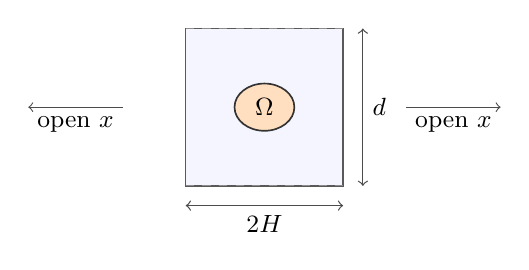
\begin{tikzpicture}[
    x=1cm,
    y=1cm,
    every node/.style={font=\small},
    strip/.style={draw=black!65, line width=0.55pt, fill=blue!4},
    inclusion/.style={draw=black!80, fill=orange!25, line width=0.6pt},
    guide/.style={draw=black!45, dashed},
    dim/.style={<->, draw=black!70, line width=0.45pt}
  ]
    \draw[strip] (-1.0,-1.0) rectangle (1.0,1.0);
    \draw[guide] (-1.0,-1.0) -- (1.0,-1.0);
    \draw[guide] (-1.0,1.0) -- (1.0,1.0);
    \draw[inclusion] (0,0) ellipse [x radius=0.38, y radius=0.30];
    \node at (0,0) {$\Omega$};

    \draw[->, draw=black!70] (-1.8,0) -- (-3.0,0);
    \draw[->, draw=black!70] (1.8,0) -- (3.0,0);
    \node[below] at (-2.4,0) {open \(x\)};
    \node[below] at (2.4,0) {open \(x\)};

    \draw[dim] (1.25,-1.0) -- (1.25,1.0);
    \node[right] at (1.25,0) {$d$};

    \draw[dim] (-1.0,-1.25) -- (1.0,-1.25);
    \node[below] at (0,-1.25) {\(2H\)};
  \end{tikzpicture}

  \vspace{0.4em}
  \small
  In this overview, the prototype is relabeled to match the line-defect
  convention: \(y\) is quasiperiodic with period \(d\), while \(x\) is the
  open direction. The prototype replaces the periodic half-leads by
  homogeneous open space on both sides of the artificial MFS boundary. Here
  \(H\) denotes the half-width of that computational boundary, not a physical
  lead period.
\end{frame}

\begin{frame}{Prototype PDE and Transmission Setting}
  For the plotted unit-cell experiment, the exterior/background and
  inclusion fields satisfy
  \[
    (\Delta+k^2)u_e=0
    \quad\text{in the background},
  \]
  \[
    (\Delta+n^2k^2)u_i=0
    \quad\text{inside the inclusion}.
  \]
  On the inclusion boundary \(\Sigma=\partial\Omega\),
  \[
    u_e=u_i,
    \qquad
    \partial_\nu u_e=\partial_\nu u_i.
  \]
  The exterior Green function enforces the quasiperiodic condition
  \[
    u(x,y+d)=e^{\ii\beta d}u(x,y)
  \]
  across the transverse period \(d\). Outside the dielectric inclusion
  \(\Omega\), the medium is the same homogeneous background everywhere.
\end{frame}

\begin{frame}{Geometry and Material Parameters}
  \footnotesize
  Parameters read from \texttt{waveguide\_1d/tep\_scan\_global2.m},
  \texttt{waveguide\_1d/tep\_plot\_band.m}, and \texttt{geom.construct\_cont}.
  \vspace{0.2em}

  \begin{center}
  \renewcommand{\arraystretch}{1.08}
  \begin{tabular}{ll}
    \hline
    quantity & value used in the plotted scripts\\
    \hline
    geometry flag & \texttt{ellipse}\\
    ellipse semi-axes & \(a=b=0.4\) by default in \texttt{geom.construct\_cont}\\
    quasiperiodic period & \(d=1.0\) in this presentation convention\\
    open-window parameter & \(H=0.5d\) in the plotted setup\\
    refractive-index ratio & \(n=\sqrt{13}\), since \texttt{er}=13\\
    wavenumbers & \(k_e=k,\quad k_i=nk\)\\
    boundary discretization & \(n_{\mathrm{tot}}=40,60,100\) in fixed-\(\beta\) scan\\
    proxy plane-wave order & \(M_{\mathrm{pw}}=10\), modes \(-10{:}10\)\\
    proxy collocation & \(N_{\mathrm{side}}=50,\ N_{\mathrm{top}}=50,\ N_{\mathrm{proxy\ edge}}=30\)\\
    \hline
  \end{tabular}
  \end{center}
  \vspace{0.1em}
  \(H\) controls the finite computational window / MFS source placement in
  the homogeneous open direction; it is not a physical lead period and is
  unrelated to \(L_\pm\).
\end{frame}

\begin{frame}{Scan Parameters for the Two Figures}
  \small
  \begin{block}{Fixed-\(\beta\) recursive refinement}
    From \texttt{tep\_scan\_global2.m}:
    \[
      d=1,\qquad \beta=\pi/d=\pi,\qquad
      k\in[0.01\beta,0.99\beta].
    \]
    Coarse grid: \(400\) samples at \(n_{\mathrm{tot}}=40\).
    Refinement uses \(n_{\mathrm{tot}}=60,100\), local grids of \(11\)
    points, and levels \(6\) through \(8\).
  \end{block}

  \begin{block}{Multi-\(\beta\) scan}
    From \texttt{tep\_plot\_band.m}:
    \[
      \beta\in[0,\pi/d]=[0,\pi],
      \qquad
      k\in[0,\pi],
    \]
    with the effective constraint \(10^{-6}\le k\le\beta-10^{-6}\).
    The script uses \(80\) beta samples, coarse \(k\)-grid size \(250\),
    and \texttt{ntot\_list(1:2)} \(=[40,60]\).
  \end{block}
\end{frame}

\begin{frame}{Quasiperiodic Green Function}
  In the displayed convention, \(d\) is the \(y\)-quasiperiodic period and
  \(x\) is the open direction:
  \[
    G_{\mathrm{QP}}^{(k)}(x,y;x_s,y_s)
    =
    \frac{\ii}{2d}
    \sum_{m\in\mathbb Z}
    \frac{1}{\gamma_m}
    e^{\ii\beta_m(y-y_s)}
    e^{\ii\gamma_m|x-x_s|},
  \]
  where
  \[
    \beta_m=\beta+\frac{2\pi m}{d},
    \qquad
    \gamma_m=\sqrt{k^2-\beta_m^2},
    \qquad \operatorname{Im}\gamma_m\ge 0.
  \]
  The decay or propagation of Rayleigh orders is controlled by \(\gamma_m\).
\end{frame}

\begin{frame}{Why the 1D Prototype Scans Below the Light Line}
  The plotted 1D prototype is designed to find guided or bound-type modes
  of a homogeneous Rayleigh exterior below the light line.
  With the first Brillouin-zone convention
  \[
    0\le\beta\le\frac{\pi}{d},
  \]
  the smallest shifted tangential wavenumber is
  \[
    \min_m|\beta_m|=\beta.
  \]
  Therefore
  \begin{block}{All Rayleigh orders evanescent}
    \[
      \boxed{
      \text{all Rayleigh orders decay}
      \iff
      k<\min_m|\beta_m|=\beta
      }
    \]
  \end{block}
\end{frame}

\begin{frame}{What Is Being Scanned Below the Light Line}
  In this prototype, the scan avoids radiating Rayleigh orders:
  \[
    k<\beta
    \quad\Longrightarrow\quad
    \gamma_m\ \text{is imaginary for every retained order }m.
  \]
  This is why the numerical experiments restrict to the region below the
  light line instead of scanning the radiating regime.
  \begin{alertblock}{Do not transfer this rule to periodic leads}
    The \(k<\beta\) criterion belongs to the homogeneous Rayleigh exterior.
    For a periodic lead, decay is decided by \(|\lambda_j(k,\beta)|\), after
    solving the one-cell Floquet trace eigenproblem.
  \end{alertblock}
\end{frame}

\begin{frame}{Layer Potentials and \(A_{\mathrm{QP}}\)}
  For a dielectric boundary \(\Sigma\), use densities
  \[
    \eta=\begin{bmatrix}\tau\\-\sigma\end{bmatrix}.
  \]
  A typical exterior representation is
  \[
    u^e
    =
    D_{\mathrm{QP}}^{(k_e)}[\tau]
    +
    S_{\mathrm{QP}}^{(k_e)}[\sigma].
  \]
  The M\"uller matrix is the boundary transmission operator
  \[
    \begin{bmatrix}
      u^+ - u^-\\
      u_n^+ - u_n^-
    \end{bmatrix}
    =
    A_{\mathrm{QP}}\eta .
  \]
  This matrix is local to the obstacle boundary \(\Sigma\).
\end{frame}

\begin{frame}{Do Not Confuse \(A_{\mathrm{QP}}\) and \(\mathcal A\)}
  The matrix
  \[
    A_{\mathrm{QP}}
  \]
  is the M\"uller matrix on the obstacle boundary \(\Sigma\).
  It enforces the material transmission condition there.
  \[
    A_{\mathrm{QP}}\eta
    =
    \text{boundary mismatch on }\Sigma .
  \]
  The full trace-matching matrix is instead
  \[
    \mathcal A.
  \]
  It contains the M\"uller row, center Rayleigh coefficients, port equations, and the outgoing Floquet trace condition.
\end{frame}

\begin{frame}{TEP Scan Objective}
  The simple 1D periodic waveguide TEP scan uses
  \[
    k_i=n k_e,
    \qquad
    A_{\mathrm{QP}}=A_{\mathrm{QP}}(k_e,k_i,\beta).
  \]
  Candidate transmission eigenvalues are detected by singular-value dips:
  \[
    k \mapsto \sigmin\!\left(A_{\mathrm{QP}}(k,\beta)\right).
  \]
  Here \(A_{\mathrm{QP}}(k,\beta)\) is the all-Kress M\"uller / QP BIE
  matrix on the inclusion boundary for one periodic unit cell.
  Numerical pipeline:
  \begin{enumerate}
    \item construct geometry and quadrature;
    \item assemble \(A_{\mathrm{QP}}\);
    \item compute \(\sigmin(A_{\mathrm{QP}})\);
    \item refine intervals around detected dips.
  \end{enumerate}
\end{frame}

\begin{frame}{Fixed-\(\beta\) Recursive Refinement Scan}
  \begin{columns}[T,onlytextwidth]
    \begin{column}{0.66\textwidth}
      \centering
      \SafeIncludeGraphics[width=\linewidth,height=0.64\textheight,keepaspectratio]{figs/tep_scan_fixed_beta.png}
    \end{column}
    \begin{column}{0.31\textwidth}
      \footnotesize
      Fixed-\(\beta\) scan from \texttt{tep\_scan\_global2.m}.
      Parameters: \(\beta=\pi\), \(d=1\), \(n=\sqrt{13}\).
      The inclusion is the default \texttt{ellipse} geometry with
      semi-axes \(a=b=0.4\).
      Recursive refinement samples narrower intervals around dips of
      \(\sigma_{\min}(A_{\mathrm{QP}}(k,\beta))\).
      The scanned interval is \(k\in[0.01\pi,0.99\pi]\).
    \end{column}
  \end{columns}
\end{frame}

\begin{frame}{Multi-\(\beta\) Singular-value Landscape}
  \begin{columns}[T,onlytextwidth]
    \begin{column}{0.66\textwidth}
      \centering
      \SafeIncludeGraphics[width=\linewidth,height=0.64\textheight,keepaspectratio]{figs/tep_plot_band.png}
    \end{column}
    \begin{column}{0.31\textwidth}
      \footnotesize
      Multi-\(\beta\) scan from \texttt{tep\_plot\_band.m}.
      Parameters: \(\beta\in[0,\pi]\), \(k\in[0,\pi]\), \(d=1\).
      The effective scan clips to
      \(10^{-6}\le k\le\beta-10^{-6}\).
      The plotted value is \(\log_{10}\sigma_{\min}(A_{\mathrm{QP}}(k,\beta))\).
    \end{column}
  \end{columns}
\end{frame}

\begin{frame}{Placeholder: Singular-value Scan Figure}
  \begin{center}
    \SafeIncludeGraphics[width=0.85\textwidth,height=0.68\textheight,keepaspectratio]{figs/sigma_scan.pdf}
  \end{center}
  \begin{itemize}
    \item No numerical values are asserted on this slide.
    \item Intended source: validated MATLAB scan output.
  \end{itemize}
\end{frame}

\section{Lead Scattering}

\begin{frame}{Lead Incoming Forcing}
  In a lead scattering problem,
  \[
    p_{\mathrm{in}}^-,
    \qquad
    p_{\mathrm{in}}^+
  \]
  are prescribed incoming coefficients.
  They define legal incoming port traces:
  \[
    D_{\mathrm{in}}^\pm p_{\mathrm{in}}^\pm,
    \qquad
    N_{\mathrm{in}}^\pm p_{\mathrm{in}}^\pm.
  \]
  The forcing is therefore not an arbitrary wall trace.
\end{frame}

\begin{frame}{Unknown Outgoing Scattered Coefficients}
  The unknown scattered field in the half-leads is represented by outgoing coefficients
  \[
    r^-,
    \qquad
    r^+.
  \]
  The corresponding outgoing trace vectors are
  \[
    D_s^\pm=D_{\mathrm{out}}^\pm r^\pm,
    \qquad
    N_s^\pm=N_{\mathrm{out}}^\pm r^\pm.
  \]
  The physical radiation condition is encoded by the selected outgoing Floquet trace basis.
\end{frame}

\begin{frame}{Empty-defect / Missing-column Field}
  In the empty center cell, the field is a homogeneous Rayleigh expansion:
  \[
    u_h(x,y)
    =
    \sum_m a_m e^{\ii\gamma_m(x-X_-)}\psi_m(y)
    +
    \sum_m b_m e^{-\ii\gamma_m(x-X_-)}\psi_m(y).
  \]
  Here \(a=(a_m)\) and \(b=(b_m)\) are right-going and left-going center-cell Rayleigh coefficients.
  They carry no plus/minus superscripts because they are not attached to positive or negative half-leads.
\end{frame}

\begin{frame}{Empty-defect Port Traces}
  With
  \[
    \Gamma=\operatorname{diag}(\gamma_m),
    \qquad
    E=\operatorname{diag}(e^{\ii\gamma_mL_0}),
  \]
  the port traces are
  \[
    D_h^- = a + b,
    \qquad
    N_h^- = -\ii\Gamma(a-b),
  \]
  \[
    D_h^+ = Ea + E^{-1}b,
    \qquad
    N_h^+ = \ii\Gamma(Ea-E^{-1}b).
  \]
\end{frame}

\begin{frame}{Port Matching at High Level}
  The scattering split is
  \[
    \text{center trace}
    =
    \text{known incoming trace}
    +
    \text{unknown outgoing scattered trace}.
  \]
  Therefore,
  \[
    D_h^\pm
    =
    D_{\mathrm{in}}^\pm p_{\mathrm{in}}^\pm
    +
    D_{\mathrm{out}}^\pm r^\pm,
  \]
  \[
    N_h^\pm
    =
    N_{\mathrm{in}}^\pm p_{\mathrm{in}}^\pm
    +
    N_{\mathrm{out}}^\pm r^\pm.
  \]
  The unknowns are the center Rayleigh coefficients and the outgoing lead coefficients.
\end{frame}

\begin{frame}{Placeholder: Bloch Multiplier Distribution}
  \begin{center}
    \SafeIncludeGraphics[width=0.85\textwidth,height=0.68\textheight,keepaspectratio]{figs/bloch_multiplier_distribution.pdf}
  \end{center}
  \begin{itemize}
    \item Mark \(|\lambda|=1\) as a reference circle.
    \item Use code-validated mode selection before inserting the figure.
  \end{itemize}
\end{frame}

\section{Center Obstacle}

\begin{frame}{New Center-obstacle Unknown}
  With an obstacle \(\Omega_0\) in \(\Ccell^0\), introduce the boundary density
  \[
    \eta=
    \begin{bmatrix}
      \tau\\-\sigma
    \end{bmatrix}.
  \]
  This density lives on
  \[
    \Sigma=\partial\Omega_0.
  \]
  The full unknown vector will also contain center Rayleigh amplitudes and outgoing lead coefficients.
\end{frame}

\begin{frame}{M\"uller BIE on \(\Sigma\)}
  The center exterior field is decomposed as
  \[
    u_e=u_h+u_s^e,
  \]
  where \(u_h\) is the center homogeneous Rayleigh field and \(u_s^e\) is generated by \(\eta\).
  The transmission condition on \(\Sigma\) gives the forced M\"uller row
  \[
    A_{\mathrm{QP}}\eta
    +
    H_\Sigma^a a
    +
    H_\Sigma^b b
    =
    0.
  \]
  This is the obstacle-boundary part of the final system.
\end{frame}

\begin{frame}{Port Matching on \(\Gamma_\pm\)}
  On the artificial boundaries, the center trace must match the half-lead trace:
  \[
    D_h^\pm+D_s^\pm
    =
    D_{\mathrm{in}}^\pm p_{\mathrm{in}}^\pm
    +
    D_{\mathrm{out}}^\pm r^\pm,
  \]
  \[
    N_h^\pm+N_s^\pm
    =
    N_{\mathrm{in}}^\pm p_{\mathrm{in}}^\pm
    +
    N_{\mathrm{out}}^\pm r^\pm.
  \]
  This is where the Bloch exterior condition enters the center-cell solve.
\end{frame}

\begin{frame}{Obstacle Density Contribution at Ports}
  The center obstacle density produces outgoing Rayleigh coefficients at the two ports:
  \[
    s^- = F_-\eta,
    \qquad
    s^+ = F_+\eta.
  \]
  Therefore
  \[
    D_s^- = F_-\eta,
    \qquad
    N_s^- = \ii\Gamma F_-\eta,
  \]
  \[
    D_s^+ = F_+\eta,
    \qquad
    N_s^+ = \ii\Gamma F_+\eta.
  \]
  These terms couple the M\"uller density to the port equations.
\end{frame}

\begin{frame}{Conceptual Block System}
  Use the unknown vector
  \[
    x=
    \begin{bmatrix}
      \eta\\ a\\ b\\ r^-\\ r^+
    \end{bmatrix}.
  \]
  The coupled trace-matching system is
  \[
    \Atr x=b_{\mathrm{in}}.
  \]
  Conceptually,
  \[
    \Atr
    =
    \begin{bmatrix}
      \text{M\"uller BIE on }\Sigma
      &
      \text{center Rayleigh forcing}
      &
      0
      \\
      \text{port traces from }\eta
      &
      \text{center Rayleigh traces}
      &
      \text{outgoing Floquet trace condition}
    \end{bmatrix}.
  \]
\end{frame}

\begin{frame}{Full Block Formula}
  \scriptsize
  In the notation of the latest formulation,
  \[
    \Atr
    =
    \begin{bmatrix}
      \Aqp & H_\Sigma^a & H_\Sigma^b & 0 & 0\\
      F_- & I & I & -D_{\mathrm{out}}^- & 0\\
      \ii\Gamma F_- & -\ii\Gamma & \ii\Gamma & -N_{\mathrm{out}}^- & 0\\
      F_+ & E & E^{-1} & 0 & -D_{\mathrm{out}}^+\\
      \ii\Gamma F_+ & \ii\Gamma E & -\ii\Gamma E^{-1} & 0 & -N_{\mathrm{out}}^+
    \end{bmatrix}.
  \]
  The right-hand side contains only legal incoming port trace data:
  \[
    b_{\mathrm{in}}
    =
    \begin{bmatrix}
      0\\
      D_{\mathrm{in}}^-p_{\mathrm{in}}^-\\
      N_{\mathrm{in}}^-p_{\mathrm{in}}^-\\
      D_{\mathrm{in}}^+p_{\mathrm{in}}^+\\
      N_{\mathrm{in}}^+p_{\mathrm{in}}^+
    \end{bmatrix}.
  \]
\end{frame}

\begin{frame}{Placeholder: Scattering Field Contour}
  \begin{center}
    \SafeIncludeGraphics[width=0.85\textwidth,height=0.68\textheight,keepaspectratio]{figs/scattering_field_contour.pdf}
  \end{center}
  \begin{itemize}
    \item Mask dielectric interiors if the interior reconstruction is not shown.
    \item Report the residual of \(\Atr x-b_{\mathrm{in}}\) with the figure.
  \end{itemize}
\end{frame}

\section{Summary}

\begin{frame}{Summary}
  \begin{itemize}
    \item Floquet trace eigenvectors come from one-cell trace propagation in the periodic lead.
    \item Rayleigh wall functions provide trace coordinates, not the physical mode basis.
    \item \(A_{\mathrm{QP}}\) is the M\"uller matrix on \(\Sigma\); \(\Atr\) is the full trace-matching matrix.
    \item Empty-defect scattering uses center Rayleigh coefficients and an outgoing Floquet trace condition.
    \item The center-obstacle problem adds the density \(\eta=[\tau;-\sigma]\) and a M\"uller BIE row.
  \end{itemize}
\end{frame}

\begin{frame}{Next Steps}
  \begin{enumerate}
    \item Validate center-obstacle scattering residuals for selected incoming port traces.
    \item Insert verified singular-value scan and multiplier figures.
    \item Compare empty-defect and center-obstacle formulations.
    \item Extend toward linear-defect crystal trace-mode analysis and full numerical validation.
  \end{enumerate}
\end{frame}

\end{document}
